\chapter{Metodología}

\section{Especificaciones Hardware y Software}

Para dar contexto a los costes computacionales asociados a los algoritmos, así como al tiempo empleado durante los experimentos, a continuación se detalla el entorno utilizado para las ejecuciones del proyecto.

En cuanto al hardware, el equipo cuenta con un procesador Intel Core i5-12500H de 12\textsuperscript{a} generación y 16 GB de memoria RAM. A nivel de sistema operativo, se ha utilizado una distribución GNU/Linux, concretamente Ubuntu 24.04.4 LTS.

En cuanto al software, el proyecto se ha desarrollado íntegramente en Python \cite{python} (versión 3.13.9). Para la ejecución de los EAs se ha utilizado \texttt{pymoo} \cite{pymoo}, un marco de optimización de código abierto. La elección de \texttt{pymoo} como marco principal de trabajo se justifica por su orientación específica hacia la investigación en MOEAs y MaOEAs, y su arquitectura orientada a objetos. Esta característica ha sido fundamental para el desarrollo del proyecto, ya que ha permitido implementar estrategias de inicialización poblacional como las técnicas voraces y modelar el problema de la selección de etiquetas SNP extendiendo las clases base de la librería.

Por otra parte, para el procesamiento de los datos genéticos y el análisis estadístico, el proyecto se apoya en librerías científicas estándar como \texttt{numpy} \cite{numpy} y \texttt{pandas} \cite{pandas}.

Adicionalmente, la generación de representaciones gráficas, como los diagramas de Frentes de Pareto, se ha llevado a cabo mediante la librería de visualización \texttt{matplotlib} \cite{matplotlib}.

\section{Definición del problema}

Tal y como se ha expuesto en los capítulos introductorios, la selección de etiquetas SNP plantea un desafío computacional extremo al ser considerado matemáticamente como un problema de optimización combinatoria análogo a la Cobertura de Conjuntos o \textit{Set Cover Problem} \cite{bafna2003haplotypes}. Para abordar este problema mediante EAs, resulta indispensable asentar previamente las bases del entorno de experimentación. A tal efecto, a lo largo de esta sección se define la procedencia del conjunto de datos, se explican conceptos básicos, se formula matemáticamente la lógica de distinguibilidad que rige el problema, se detalla el preprocesamiento de filtrado y, finalmente, se establece la representación cromosómica que codificará a los individuos.

\subsection{Dataset}
El núcleo de las ejecuciones de este proyecto se fundamenta en el conjunto de datos propuesto por Hinds \textit{et al.} \cite{hinds2005whole}, un referente estándar para el estudio de patrones de variación de ADN a nivel genómico en poblaciones humanas. Este \textit{dataset} cataloga la variación genética de tres poblaciones globales, recopilando secuencias de más de un millón de SNPs \cite{bafna2003haplotypes}. En el contexto de este proyecto, se ha aislado un bloque genómico compuesto originariamente por 1032 SNPs, proporcionando un entorno de prueba real y representativo para evaluar los algoritmos. Cabe destacar que este mismo fragmento genético poblacional fue el empleado en el estudio de Ting \textit{et al.} \cite{ting2010multi}, lo que permite enmarcar el experimento dentro de los estándares de la literatura. 

\subsection{Matriz de haplotipos y etiquetas SNP}
Para ilustrar de forma visual cómo se estructuran estos datos y cómo operan los algoritmos sobre ellos, se expone a continuación una matriz binaria (véase la matriz \ref{eq:matriz_H}). 

\begin{equation}\label{eq:matriz_H}
\begin{array}{cc}
 & \begin{array}{cccccc}
 \text{\scriptsize 1} & \text{\scriptsize 2} & \text{\scriptsize 3} & \text{\scriptsize 4} & \text{\scriptsize 5} & \text{\scriptsize 6}
 \end{array} \\
 \begin{array}{c} h_1 \\ h_2 \\ h_3 \\ h_4 \end{array} &
 \left(\begin{array}{cccccc}
 0 & 0 & 0 & 1 & 0 & 1 \\
 0 & 0 & 0 & 0 & 0 & 0 \\
 0 & 1 & 0 & 1 & 1 & 1 \\
 0 & 1 & 0 & 0 & 1 & 0 
 \end{array}\right)
\end{array}
\end{equation}

Esta matriz, diseñada con fines didácticos, está formada por 4 secuencias (filas) y 6 SNPs (columnas). En esta estructura matemática, las columnas representan las posiciones concretas en la cadena de ADN, mientras que las filas representan los haplotipos. Biológicamente, un haplotipo se define como una combinación específica de alelos que tienden a heredarse juntos en un único cromosoma \cite{bafna2003haplotypes}.

Por otra parte, un etiqueta SNP se define como un polimorfismo representativo (es decir, una variación específica en la secuencia de ADN) que, al actuar en conjunto con otros etiquetas SNP, permite capturar la variación genética de un bloque de haplotipos sin necesidad de secuenciarlos en su totalidad \cite{bafna2003haplotypes, ting2010multi}. Al seleccionar únicamente estos SNPs representativos, se logra reducir drásticamente la dimensionalidad de los datos originales. 

\subsection{Distinguibilidad}
Sin embargo, el concepto matemático central que rige la validez de estas columnas seleccionadas es la \textit{distinguibilidad} \cite{bafna2003haplotypes}. Dos haplotipos de la matriz se consideran distinguibles si difieren en al menos una posición alélica. Por consiguiente, el objetivo de la búsqueda de etiquetas SNP es encontrar un subconjunto de columnas lo más reducido posible que garantice que todos los pares de haplotipos que eran distinguibles en la matriz original sigan siéndolo reduciéndola a la matriz de los etiquetas SNP.

Observando la matriz \ref{eq:matriz_H}, los cuatro haplotipos son únicos y, por tanto, distinguibles entre sí. Si un algoritmo evaluase esta matriz, podría determinar que aislando únicamente las columnas 2 y 4 (es decir, seleccionando $\text{SNP}_2$ y $\text{SNP}_4$), se pueden representar todos los haplotipos. Esto es debido a que el $\text{SNP}_2$ distingue a los pares de haplotipos con alelos opuestos en dicha columna (los pares $(h_1, h_3)$, $(h_1, h_4)$, $(h_2, h_3)$ y $(h_2, h_4)$); sin embargo, no logra distinguir los pares $(h_1, h_2)$ ni $(h_3, h_4)$, por lo que es necesario seleccionar otro SNP complementario. Al seleccionar el $\text{SNP}_4$, se consiguen distinguir esos pares restantes ($(h_1, h_2)$ y $(h_3, h_4)$). De forma aislada, el $\text{SNP}_4$ no es capaz de distinguir los pares $(h_1, h_3)$ ni $(h_2, h_4)$, pero esto deja de ser un problema porque ya lo hacía el $\text{SNP}_2$. De este modo, al combinar ambas columnas, se ha logrado mantener el $100\%$ de la distinguibilidad original utilizando solo 2 de las 6 columnas disponibles. Ese subconjunto óptimo conformaría el conjunto de etiquetas SNP (donde tanto el $\text{SNP}_2$ como el $\text{SNP}_4$ son etiquetas SNP individuales que forman la solución conjunta), generando la submatriz resultante (véase la matriz \ref{eq:matriz_tag}):

\begin{equation}\label{eq:matriz_tag}
\begin{array}{cc}
 & \begin{array}{cc}
 \text{\scriptsize 2} & \text{\scriptsize 4}
 \end{array} \\
 \begin{array}{c} h_1 \\ h_2 \\ h_3 \\ h_4 \end{array} &
 \left(\begin{array}{cc}
 0 & 1 \\
 0 & 0 \\
 1 & 1 \\
 1 & 0 
 \end{array}\right)
\end{array}
\end{equation}

\subsection{Preprocesamiento: Eliminación de SNPs monomórficos}
Con el objetivo de delimitar el dominio de los algoritmos y evitar el procesamiento de ruido estadístico, el conjunto original fue sometido a una etapa de preprocesamiento, al igual que se implementó en el código fuente de Ting \textit{et al.} \cite{ting2010multi}. Dicha limpieza consistió en la eliminación de los SNPs monomórficos. Para visualizar cómo funciona este filtrado sobre el ejemplo, se puede comprobar que el $\text{SNP}_1$ y el $\text{SNP}_3$ (primera y tercera columna de la matriz \ref{eq:matriz_H}) son secuencias monomórficas conformadas íntegramente por ceros. Dado que presentan el mismo alelo en todos los individuos de la muestra, carecen de variabilidad genética y no aportan ninguna distinguibilidad, por lo que el algoritmo de preprocesamiento las elimina. Esto da como resultado una matriz filtrada más compacta (véase la matriz \ref{eq:matriz_H_prima}):

\begin{equation}\label{eq:matriz_H_prima}
\begin{array}{cc}
 & \begin{array}{cccc}
 \text{\scriptsize 2} & \text{\scriptsize 4} & \text{\scriptsize 5} & \text{\scriptsize 6}
 \end{array} \\
 \begin{array}{c} h_1 \\ h_2 \\ h_3 \\ h_4 \end{array} &
 \left(\begin{array}{cccc}
 0 & 1 & 0 & 1 \\
 0 & 0 & 0 & 0 \\
 1 & 1 & 1 & 1 \\
 1 & 0 & 1 & 0 
 \end{array}\right)
\end{array}
\end{equation}

Aplicando este mismo principio de filtrado masivo al bloque completo de 1032 SNPs de Hinds \textit{et al.} \cite{hinds2005whole}, se logró purgar el ruido y reducir la cadena a un total de $n = 772$ SNPs polimórficos efectivos. Este tamaño de entrada determina la longitud de los individuos con los que trabajarán los algoritmos del estudio.

\subsection{Representación cromosómica de las soluciones}
Desde la perspectiva de las estructuras de datos, la representación genética de una posible solución (o individuo) dentro de los algoritmos se ha modelado como un vector binario unidimensional de tamaño fijo, siguiendo la codificación habitual de la literatura para este problema (como hizo Ting \textit{et al.} \cite{ting2010multi} o el estudio base de Moqa \textit{et al.} \cite{moqa2022assessing}):

\[ 
x = (x_1, x_2, \dots, x_n) \quad \text{donde} \quad x_i \in \{0, 1\} \text{ y } n = 772 
\]

En esta codificación booleana, si la posición $x_i$ toma el valor $1$, significa que el $i$-ésimo SNP de la cadena ha sido seleccionado como parte del subconjunto final (etiqueta SNP); si toma el valor $0$, el SNP es descartado de la solución.

Esta formulación permite definir la magnitud del espacio de búsqueda ($\Omega$). Para el conjunto filtrado, la dimensión del espacio combinatorio sobre el que operarán los algoritmos es exactamente:
\[ 
|\Omega| = 2^{772} 
\]

\section{Objetivos Absolutos y Proporcionales}

Para evaluar la aptitud de un subconjunto de etiquetas SNP candidato \cite{ting2010multi}, denotado computacionalmente como la solución $X$, el problema define cuatro funciones objetivo.

Para definir estas funciones, sea $\mathcal{H}$ el conjunto total de haplotipos de la población y $P$ el número total de pares de haplotipos posibles, definido como $P = \frac{|\mathcal{H}|(|\mathcal{H}|-1)}{2}$. Asimismo, se define $D_{i,j}(X)$ como la distancia de Hamming entre el haplotipo $i$ y el haplotipo $j$, calculada evaluando únicamente los SNPs que pertenecen al subconjunto seleccionado $X$ (individuo cromosómico).

Este TFG estudia y compara dos modelos matemáticos distintos: una formulación absoluta (propuesta originalmente en este trabajo, aunque inspirada conceptualmente en las funciones objetivo de Ting \textit{et al.} \cite{ting2010multi} y Moqa \textit{et al.} \cite{moqa2022assessing}) y una formulación proporcional (implementada explícitamente por dichos autores). A continuación se definen formalmente ambos enfoques.

\subsection{Formulación Absoluta}
Como punto de partida metodológico para los experimentos, se establece una formulación matemática que en este trabajo se denominará \textit{absoluta}. Este enfoque evalúa la calidad de la solución utilizando directamente los valores brutos de las distancias de Hamming. Los cuatro objetivos a optimizar se definen de la siguiente manera:

\begin{itemize}
    \item \textbf{$f_1$ (Compacidad):} Mide el tamaño físico y el coste económico del panel genético, representado por el número total de SNPs seleccionados en la solución $X$. Su objetivo es la minimización:
    \begin{equation}
        f_1(X) = |X|
    \end{equation}
    
    \item \textbf{$f_2$ (Tolerancia):} Se define como la peor distancia de Hamming encontrada entre cualquier par de haplotipos de la muestra. Su maximización asegura que todos los individuos sean distinguibles entre sí, proporcionando un margen de fallos en el laboratorio equivalente a $f_2(X) - 1$.
    \begin{equation}
        f_2(X) = \min_{1 \le i < j \le |\mathcal{H}|} D_{i,j}(X)
    \end{equation}
    
    \item \textbf{$f_3$ (Disimilitud):} Cuantifica la capacidad de distinción general que proporciona la solución $X$ evaluando la distancia media de Hamming de toda la población. Su objetivo es la maximización:
    \begin{equation}
        f_3(X) = \mu_{D}(X) = \frac{1}{P} \sum_{1 \le i < j \le |\mathcal{H}|} D_{i,j}(X)
    \end{equation}
    
    \item \textbf{$f_4$ (Balance):} Mide la desviación de las distancias de Hamming respecto a la media. La minimización de esta varianza busca evitar sesgos, logrando que la capacidad de distinción esté equitativamente distribuida y ningún par acapare la diferenciación.
    \begin{equation}
        f_4(X) = \sigma^2_{D}(X) = \frac{1}{P} \sum_{1 \le i < j \le |\mathcal{H}|} \left( D_{i,j}(X) - f_3(X) \right)^2
    \end{equation}
\end{itemize}

\subsection{Formulación Proporcional}
Esta formulación sigue la literatura de referencia establecida por Ting \textit{et al.} \cite{ting2010multi} y Moqa \textit{et al.} \cite{moqa2022assessing}, en la que los objetivos de compacidad ($f_1$) y tolerancia ($f_2$) se mantienen idénticos, mientras que, por algún motivo no explicado en dichos estudios, la disimilitud ($f_3$) y el balance ($f_4$) se normalizan dividiéndolos por $f_1(X)$ y $f_1(X)^2$ respectivamente:

\begin{equation}
    f_3^{\text{prop}}(X) = \frac{f_3(X)}{f_1(X)}
\end{equation}

\begin{equation}
    f_4^{\text{prop}}(X) = \frac{f_4(X)}{f_1(X)^2}
\end{equation}

\subsection{Transformación a minimización}
Por defecto, la librería \texttt{pymoo} requiere que todos los objetivos del problema sean de minimización \cite{pymoo}. Para adaptar el código a este requisito sin alterar el espacio de objetivos original, las funciones que deben ser maximizadas ($f_2$ y $f_3$) se someten a una transformación matemática estándar por negación ($f' = -f$) \cite{deb2001multiobjective}. De este modo, los algoritmos operan internamente sobre:

\begin{equation}
    f'_2(X) = -f_2(X) \quad \text{y} \quad f'_3(X) = -f_3(X)
\end{equation}

\subsection{Factibilidad de individuos}
Para que una solución $X$ sea válida (factible) desde el punto de vista biológico, debe garantizar como mínimo que, en la submatriz de etiquetas SNP, todos los pares de haplotipos (filas) presenten al menos una diferencia alélica (es decir, que sigan siendo distinguibles) \cite{bafna2003haplotypes}. Matemáticamente, esto implica que la tolerancia ($f_2$) de la solución debe ser estrictamente mayor que cero ($f_2(X) \ge 1$).

Con el fin de guiar la convergencia evolutiva y forzar a los algoritmos a descartar las secuencias infactibles, se define una restricción general en forma de inecuación $G(X) \le 0$, siguiendo el marco estándar de manejo de restricciones en EAs \cite{deb2001multiobjective}:

\begin{equation}
    G(X) = 1 - f_2(X) \le 0
\end{equation}

Si un individuo genético no logra diferenciar a todos los pares ($f_2(X) = 0$), el valor de la restricción evaluada será $G(X) = 1$, infringiendo la inecuación y desencadenando una penalización algorítmica que degradará fuertemente la aptitud de la solución dentro de la población para evitar su propagación.

Para ilustrar este concepto de penalización sobre la matriz didáctica original (véase la matriz \ref{eq:matriz_H}), supóngase que el algoritmo genera un individuo $x = (0, 1, 0, 0, 0, 0)$ en el que únicamente se ha seleccionado el $\text{SNP}_2$. Tal y como se demostró empíricamente en la sección de distinguibilidad, esta columna aislada es incapaz de diferenciar los pares de haplotipos $(h_1, h_2)$ y $(h_3, h_4)$. En consecuencia, la tolerancia de este individuo será cero ($f_2(X) = 0$), lo que arrojará un valor de restricción $G(X) = 1$. Al ser mayor que cero, el modelo detectará la infracción de la inecuación y clasificará automáticamente a la solución como infactible.

\section{Fundamentos de Optimización Multiobjetivo}

En los problemas de optimización multiobjetivo, como es el caso de la selección de etiquetas SNP, se busca optimizar simultáneamente múltiples funciones que, por norma general, entran en conflicto entre sí. En este contexto matemático, no existe una única solución que sea óptima para todos los objetivos a la vez. Para determinar de forma objetiva qué soluciones son superiores durante la evolución del algoritmo, se recurre a los conceptos de Dominancia de Pareto y Frente de Pareto.

\subsection{Dominancia de Pareto}
Dadas dos soluciones factibles $A$ y $B$, se dice que la solución $A$ \textit{domina} a la solución $B$ (denotado formalmente como $A \prec B$) si se cumplen estrictamente dos condiciones \cite{deb2001multiobjective}:
\begin{enumerate}
    \item La solución $A$ no es peor que $B$ en ninguno de los objetivos evaluados.
    \item La solución $A$ es estrictamente mejor que $B$ en al menos un objetivo.
\end{enumerate}

Si $A$ domina a $B$, significa que $A$ es una solución matemáticamente superior, por lo que $B$ puede ser descartada del conjunto de soluciones candidatas a ser parte del Frente de Pareto. Cuando dos soluciones no se dominan mutuamente (por ejemplo, una es mejor en compacidad pero otra es mejor en tolerancia), ambas se consideran incomparables y se mantienen como compromisos válidos.

\subsection{Frente de Pareto}
El conjunto de todas las soluciones no dominadas descubiertas conforma el denominado Frente de Pareto \cite{zitzler1999multiobjective}. Estas soluciones representan los mejores compromisos posibles entre los distintos objetivos en conflicto.

La morfología geométrica del Frente de Pareto en el espacio objetivo varía en función de la dirección de optimización (minimización o maximización) que requiera cada función. En la Figura \ref{fig:pareto_fronts} se ilustra visualmente cómo se ubican las soluciones no dominadas (en rojo) dependiendo de si el problema exige minimizar o maximizar cada eje.

\begin{figure}[H]
    \centering
    \includegraphics[width=0.85\textwidth]{../figuras_metricas/pareto_fronts.pdf}
    \caption[Frente de Pareto bajo combinaciones de optimización]{Representación bidimensional del Frente de Pareto bajo distintas combinaciones de optimización (minimización y maximización). Los puntos rojos conforman el conjunto de soluciones no dominadas, estableciendo la frontera geométrica óptima, mientras que los puntos grises representan las soluciones dominadas subóptimas.}
    \label{fig:pareto_fronts}
\end{figure}

El propósito fundamental de un MaOEA \cite{ishibuchi2008evolutionary} es descubrir una aproximación a este Frente de Pareto que cumpla dos propiedades clave: una alta \textit{convergencia} (que las soluciones se acerquen lo máximo posible al frente óptimo teórico real\footnote{En problemas de alta dimensionalidad y vasto espacio de búsqueda, resulta computacionalmente inabarcable hallar el Frente de Pareto absoluto mediante evaluaciones de fuerza bruta. Por ello, el frente óptimo teórico real actúa como un límite matemático ideal hacia el cual los EAs intentan aproximar iterativamente sus frentes empíricos.}) y una alta \textit{diversidad} (que las soluciones se distribuyan de manera uniforme a lo largo de todo el frente, ofreciendo un catálogo completo de alternativas) \cite{bosman2003balance}.

\section{Algoritmos evolutivos seleccionados}

Para realizar un estudio comparativo exhaustivo, se ha seleccionado un conjunto diverso de EAs. Dado que el problema de selección de etiquetas SNP presenta una dimensionalidad de cuatro objetivos (catalogándose formalmente como un problema de muchos objetivos), la comparativa incorpora tanto MOEAs como MaOEAs. Concretamente, se han incluido todos los algoritmos evaluados en el estudio de referencia de Moqa \textit{et al.} \cite{moqa2022assessing}, ampliando la lista con otros adicionales para abarcar un espectro algorítmico más amplio. Esta selección final cubre diferentes paradigmas evolutivos, lo que permite analizar cómo operan sus distintas estrategias de búsqueda empleando ambas formulacines de objetivos. Los algoritmos elegidos se agrupan en las siguientes categorías:

\subsection{Algoritmos basados en dominancia de Pareto}
Este paradigma constituye el enfoque clásico, donde la presión de selección recae principalmente sobre la relación de dominancia de Pareto entre las soluciones de la población. Teóricamente, como demostró la revisión de Ishibuchi \textit{et al.} \cite{ishibuchi2008evolutionary}, cuando el problema escala a cuatro o más objetivos, casi todos los individuos de la población pasan a ser no dominados. Esto anula la presión selectiva de la relación de Pareto y obliga al algoritmo a depender de sus métricas de diversidad (como el \textit{crowding distance} de NSGA-II). 

A pesar de esta conocida limitación teórica, se incluyen algoritmos clásicos como NSGA-II o SPEA2 como elementos de control. Su propósito es doble: establecer un rendimiento base y comprobar si esa pérdida de eficacia matemática se cumple realmente en el problema de selección de etiquetas SNP \cite{ting2010multi, moqa2022assessing}.
\begin{itemize}
    \item \textbf{NSGA-II:} El algoritmo \textit{Non-dominated Sorting Genetic Algorithm II} \cite{deb2002fast} clasifica a los individuos en frentes de no dominancia y aplica un operador de distancia de agrupamiento (\textit{crowding distance}) para preservar la diversidad poblacional.
    \item \textbf{SPEA2:} El \textit{Strength Pareto Evolutionary Algorithm 2} \cite{zitzler2001spea2} mantiene un archivo secundario con las mejores soluciones encontradas durante la evolución e incorpora una técnica de estimación de densidad basada en el $k$-ésimo vecino más cercano.
\end{itemize}

\subsection{Algoritmos basados en vectores de referencia}
Dado que estos algoritmos están diseñados específicamente para lidiar con entornos MaOEA, este grupo resulta intrínsecamente idóneo para abordar el problema de cuatro funciones objetivo. Su estrategia principal radica en guiar la búsqueda hacia el frente de Pareto utilizando un conjunto de vectores de referencia distribuidos uniformemente en el espacio de objetivos.
\begin{itemize}
    \item \textbf{MOEA/D:} El \textit{Multi-Objective Evolutionary Algorithm based on Decomposition} \cite{zhang2007moea} desagrega el problema original en un conjunto de subproblemas escalares (utilizando de forma estándar la función de agregación de Tchebycheff) que se optimizan de forma colaborativa mediante la información de vecindarios.
    \item \textbf{NSGA-III:} Como evolución directa de NSGA-II, el algoritmo NSGA-III \cite{deb2013evolutionary} sustituye el cálculo de la distancia de agrupamiento por un enfoque de mantenimiento de diversidad apoyado en vectores de referencia distribuidos uniformemente, logrando escalar con eficacia en alta dimensionalidad.
    \item \textbf{U-NSGA-III:} El algoritmo \textit{Unified NSGA-III} \cite{seada2015unified} perfecciona la propuesta anterior mediante la implementación de un operador de nichos adaptativo continuo que mitiga la pérdida de control de dominancia.
    \item \textbf{RVEA:} El \textit{Reference Vector Guided Evolutionary Algorithm} \cite{cheng2016reference} introduce una estrategia de adaptación dinámica para los vectores de referencia, otorgando una convergencia más estable frente a frentes de Pareto de topología irregular.
\end{itemize}

\subsection{Algoritmos basados en indicadores de calidad}
Este paradigma alternativo evalúa la aptitud de la población reduciendo su calidad global (convergencia y diversidad) a un único valor numérico o indicador matemático, el cual guía la presión selectiva.
\begin{itemize}
    \item \textbf{SMS-EMOA:} El \textit{S-Metric Selection Evolutionary Multi-Objective Algorithm} \cite{beume2007sms} fundamenta su mecanismo de selección ambiental en la contribución marginal de cada individuo a la métrica de hipervolumen (\textit{S-metric}) para maximizar de forma holística el espacio dominado.
    \item \textbf{AGE-MOEA-II:} El \textit{Approximation-Guided Evolutionary Algorithm II} \cite{panichella2022adaptive} sustituye el hipervolumen por una puntuación de supervivencia basada en aproximación geométrica adaptativa de la topología del frente de Pareto. Ejerce una presión selectiva sumamente competitiva, reduciendo drásticamente el coste computacional.
\end{itemize}

\section{Estrategias de inicialización}

La calidad y diversidad de la población inicial resultan determinantes para la correcta convergencia de los EAs, especialmente en entornos de muchos objetivos donde el vasto espacio de búsqueda dificulta el descubrimiento rápido del frente de Pareto. Para evaluar el impacto de las soluciones iniciales en el problema de selección de etiquetas SNP, se han incorporado tres mecanismos de inicialización poblacional de distintas características:

\textbf{Inicialización aleatoria densa (\textit{random\_dense})} \\
Constituye el enfoque aleatorio estándar utilizado por Ting \textit{et al.} \cite{ting2010multi}. En este mecanismo, cada SNP tiene una probabilidad uniforme del $50\%$ de ser activado.

\begin{algorithm}[H]
\caption{Inicialización aleatoria densa (\textit{random\_dense})}
\begin{algorithmic}[1]
\Require $N$: Número total de etiquetas SNP candidatos
\Require $M$: Tamaño de la población
\Ensure Población inicial $P$
\State $P \gets \emptyset$ \Comment{Inicializa el conjunto poblacional a vacío}
\For{$i \gets 1 \textbf{ to } M$} \Comment{Itera hasta alcanzar el tamaño poblacional exigido}
    \State $individuo \gets \emptyset$ \Comment{Crea un nuevo cromosoma inicialmente sin SNPs}
    \For{$j \gets 1 \textbf{ to } N$} \Comment{Recorre secuencialmente todos los SNPs candidatos}
        \If{$\textit{random}(0, 1) < 0.5$} \Comment{Garantiza una exploración del espacio sin sesgo voraz}
            \State $individuo \gets individuo \cup \{SNP_j\}$ \Comment{Agrega el SNP actual al cromosoma si cumple la condición}
        \EndIf
    \EndFor
    \State $P \gets P \cup \{individuo\}$
\EndFor
\State \Return $P$
\end{algorithmic}
\end{algorithm}

\textbf{Inicialización voraz de Ting (\textit{greedy\_ting})} \\
Este mecanismo se fundamenta en el método voraz propuesto originalmente por Ting \textit{et al.} \cite{ting2010multi}. Su estructura es híbrida y opera en tres fases secuenciales. En primer lugar, se inyectan soluciones ancla deterministas (individuos de referencia para asegurar la presencia de los extremos del frente de Pareto en la población inicial, ya que tienen valores óptimos en algunos objetivos): una construida mediante selección voraz por balance alélico hasta cubrir todos los pares, y otra que activa todos los SNPs con perfil de cobertura único. A continuación, se genera una segunda fase inyectando individuos diversificados, alternando entre una selección voraz por grupos de cobertura idéntica (escogiendo un representante aleatorio de cada grupo hasta cubrir todos los pares) y una selección que toma exactamente un SNP por grupo sin exigir cobertura completa. Finalmente, la fracción restante de la población se rellena con individuos puramente aleatorios con probabilidad del $50\%$, aportando diversidad a la población resultante.

\begin{algorithm}[H]
\caption{Inicialización híbrida de Ting (\textit{greedy\_ting}) (Parte 1)}
\begin{algorithmic}[1]
\Require $\mathcal{H}$: Matriz de haplotipos
\Require $r$: Ratio de soluciones voraces
\Require $M$: Tamaño de la población
\Ensure Población inicial $P$
\State $P \gets \emptyset$ \Comment{Instancia la población base vacía}
\State $M_{greedy} \gets \lceil M \times r \rceil$ \Comment{Calcula el número de individuos voraces a generar}
\State $n_{ancla} \gets \lceil r \times 10 \rceil$ \Comment{Calcula el número de cromosomas ancla necesarios}
\State $orden \gets$ Lista de SNPs ordenados por proximidad a la frecuencia alélica del $50\%$, filtrando duplicados \Comment{Prioriza las mutaciones más informativas}
\State $ancla_{greedy} \gets$ Seleccionar SNPs de $orden$ (de mayor a menor balance) hasta cubrir todos los pares \Comment{Construye un ancla de baja compacidad}
\State $ancla_{densa} \gets$ Activar todos los SNPs presentes en $orden$ \Comment{Construye un ancla con alta tolerancia y distancia de hamming media}
\State 
\State \textbf{Fase 1 --- Anclas deterministas:}
\For{$i \gets 1$ \textbf{to} $\lfloor n_{ancla} / 2 \rfloor$} \Comment{Inyecta copias idénticas para estabilizar la población}
    \State $P \gets P \cup \{ancla_{greedy}\}$ \Comment{Añade el primer ancla a la población}
    \State $P \gets P \cup \{ancla_{densa}\}$ \Comment{Añade el segundo ancla}
\EndFor
\end{algorithmic}
\end{algorithm}

\addtocounter{algorithm}{-1}
\begin{algorithm}[H]
\caption{Inicialización híbrida de Ting (\textit{greedy\_ting}) (Parte 2)}
\begin{algorithmic}[1]
\State \textbf{Fase 2 --- Voraz diversificada:}
\State $grupos \gets$ Agrupar SNPs con idéntico perfil de cobertura sobre los pares \Comment{Evita evaluar mutaciones redundantes}
\While{$|P| < M_{greedy}$} \Comment{Continúa el bucle mientras falten soluciones voraces}
    \State $individuo_1 \gets \emptyset$, $cubiertos \gets \emptyset$ \Comment{Prepara un nuevo cromosoma y su registro de cobertura a cero}
    \For{cada $grupo$ en $grupos$ (orden aleatorio)}
        \If{todos los pares cubiertos} \textbf{break} \EndIf
        \State Elegir un SNP aleatorio del $grupo$, añadirlo a $individuo_1$
        \State Actualizar $cubiertos$
    \EndFor
    \State $P \gets P \cup \{individuo_1\}$
    \If{$|P| < M_{greedy}$} \Comment{Verifica si el número poblacional aún lo requiere}
        \State $individuo_2 \gets \emptyset$ \Comment{Instancia un segundo cromosoma vacío}
        \For{cada $grupo$ en $grupos$}
            \State Elegir un SNP aleatorio del $grupo$, añadirlo a $individuo_2$
        \EndFor
        \State $P \gets P \cup \{individuo_2\}$
    \EndIf
\EndWhile
\State 
\State \textbf{Fase 3 --- Relleno aleatorio:}
\While{$|P| < M$} \Comment{Se ejecuta si aún no se ha completado la población}
    \State $individuo_{rand} \gets$ Generar individuo aleatorio (probabilidad $0.5$)
    \State $P \gets P \cup \{individuo_{rand}\}$
\EndWhile
\State \Return $P$
\end{algorithmic}
\end{algorithm}


\textbf{Inicialización voraz de multitolerancia (\textit{greedy\_multi})} \\
Como aportación original de este trabajo, implementa una estrategia voraz diseñada específicamente para potenciar la tolerancia a fallos ($f_2$). Esta inicialización impone distintos niveles de tolerancia ($k$-tolerancia) a los individuos generados, distribuyendo un objetivo progresivo de tolerancia $k$ de forma lineal entre todos los individuos de la población inicial. 

A nivel algorítmico, el proceso de construcción de cada cromosoma se desarrolla iterativamente: en cada paso se calcula una puntuación dinámica para todos los SNPs candidatos, equivalente al número de pares de haplotipos insatisfechos que cada SNP es capaz de distinguir. El SNP que maximiza esta puntuación es seleccionado y los niveles de tolerancia del sistema se actualizan. Este bucle voraz continúa hasta que todos los pares alcanzan el objetivo $k$ asignado al individuo o bien, hasta que se alcanza el límite biológico de tolerancia que tiene el dataset. 

Al asignar diferentes niveles de tolerancia a cada individuo, se garantiza que la población arranque con una amplia variedad de soluciones: desde cromosomas muy ligeros ($k=1$) hasta otros con alta compacidad ($f_1$) y tolerancia ($f_2$).

\begin{algorithm}[H]
\caption{Inicialización dinámica de multitolerancia (\textit{greedy\_multi})}
\begin{algorithmic}[1]
\Require $K_{max}$: Nivel máximo de tolerancia a fallos exigido
\Require $M$: Tamaño de la población
\Require $LimitesBio$: Tolerancia máxima posible del dataset
\Ensure Población inicial $P$
\State $P \gets \emptyset$ \Comment{Declara el conjunto poblacional vacío}
\State $ObjetivosK \gets$ Secuencia lineal desde $1$ hasta $K_{max}$ de longitud $M$
\For{cada $k_{obj} \in ObjetivosK$}
    \State $individuo \gets \emptyset$
    \State $estado\_tolerancia \gets$ Vector a ceros para todos los pares
    \State $K_{real} \gets \min(k_{obj}, LimitesBio)$
    \While{existan pares con $estado\_tolerancia < K_{real}$} \Comment{Itera añadiendo SNPs hasta alcanzar la tolerancia exigida}
        \State $S^* \gets \emptyset$ \Comment{Asigna cero a la variable del mejor candidato}
        \State $max\_distinguibilidad \gets 0$ \Comment{Asigna el valor máximo a cero}
        \For{cada $SNP$ candidato no seleccionado}
            \State $distinguibilidad \gets$ Pares que este SNP distingue y aún necesitan tolerancia
            \If{$distinguibilidad > max\_distinguibilidad$}
                \State $max\_distinguibilidad \gets distinguibilidad$
                \State $S^* \gets SNP$
            \EndIf
        \EndFor
        \If{$max\_distinguibilidad == 0$} \textbf{break} \EndIf
        \State $individuo \gets individuo \cup \{S^*\}$
        \State Actualizar $estado\_tolerancia$ sumando las distinciones aportadas por $S^*$ 
    \EndWhile
    \State $P \gets P \cup \{individuo\}$
\EndFor
\State \Return $P$
\end{algorithmic}
\end{algorithm}

\section{Selección de operadores genéticos de cruce}

La fase de cruce constituye el mecanismo principal de búsqueda en los EAs, permitiendo a la población intercambiar secuencias genéticas entre distintas soluciones. Dado que el problema de selección de etiquetas SNP requiere una representación basada en codificación binaria (donde cada gen es un 1 o un 0), es obligatorio seleccionar operadores de cruce diseñados específicamente para espacios discretos. En este trabajo se han evaluado cuatro:

\begin{itemize}
    \item \textbf{Cruce de un punto (\textit{One Point Crossover} - 1P):} Constituye el operador más elemental \cite{holland1975adaptation}. Se selecciona aleatoriamente un único punto de corte a lo largo del cromosoma de los progenitores. Para generar la descendencia, el primer descendiente hereda el segmento genético anterior al punto de corte del primer progenitor y el segmento posterior del segundo progenitor, invirtiéndose la asignación para el segundo descendiente, tal y como se representa en la Figura \ref{fig:crossover_1p}. Aunque preserva la integridad de los genes que están muy juntos, presenta el problema de generar un fuerte sesgo posicional (separa con una alta probabilidad los genes de los extremos opuestos, pero tiende a mantener juntos aquellos que están más próximos entre sí).

\begin{figure}[H]
\centering
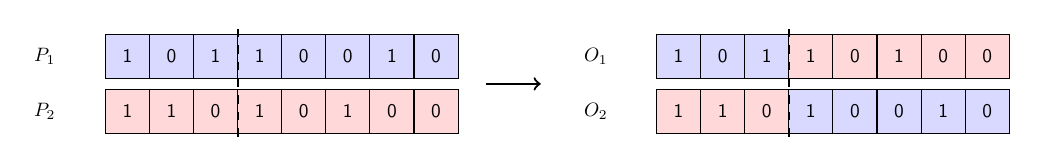
\begin{tikzpicture}[font=\sffamily, scale=0.7, transform shape]
\tikzstyle{bit}=[draw, minimum width=0.8cm, minimum height=0.8cm]
\tikzstyle{p1}=[bit, fill=blue!15]
\tikzstyle{p2}=[bit, fill=red!15]
\node at (-1.5, 1) {$P_1$};
\node[p1] at (0,1) {1}; \node[p1] at (0.8,1) {0}; \node[p1] at (1.6,1) {1}; \node[p1] at (2.4,1) {1}; \node[p1] at (3.2,1) {0}; \node[p1] at (4.0,1) {0}; \node[p1] at (4.8,1) {1}; \node[p1] at (5.6,1) {0};
\node at (-1.5, 0) {$P_2$};
\node[p2] at (0,0) {1}; \node[p2] at (0.8,0) {1}; \node[p2] at (1.6,0) {0}; \node[p2] at (2.4,0) {1}; \node[p2] at (3.2,0) {0}; \node[p2] at (4.0,0) {1}; \node[p2] at (4.8,0) {0}; \node[p2] at (5.6,0) {0};
\draw[->, thick] (6.5, 0.5) -- (7.5, 0.5);
\node at (8.5, 1) {$O_1$};
\node[p1] at (10,1) {1}; \node[p1] at (10.8,1) {0}; \node[p1] at (11.6,1) {1}; \node[p2] at (12.4,1) {1}; \node[p2] at (13.2,1) {0}; \node[p2] at (14.0,1) {1}; \node[p2] at (14.8,1) {0}; \node[p2] at (15.6,1) {0};
\node at (8.5, 0) {$O_2$};
\node[p2] at (10,0) {1}; \node[p2] at (10.8,0) {1}; \node[p2] at (11.6,0) {0}; \node[p1] at (12.4,0) {1}; \node[p1] at (13.2,0) {0}; \node[p1] at (14.0,0) {0}; \node[p1] at (14.8,0) {1}; \node[p1] at (15.6,0) {0};
\draw[dashed, thick] (2.0, 1.5) -- (2.0, -0.5);
\draw[dashed, thick] (12.0, 1.5) -- (12.0, -0.5);
\end{tikzpicture}
\caption{Ejemplo de funcionamiento del Cruce de un punto (1P).}
\label{fig:crossover_1p}
\end{figure}

    \item \textbf{Cruce de dos puntos (\textit{Two Point Crossover} - 2P):} Extensión del cruce anterior \cite{dejong1975analysis} en la que se definen aleatoriamente dos puntos de corte en el cromosoma. La recombinación se produce intercambiando exclusivamente el material genético situado entre ambos puntos, según se muestra en el esquema de la Figura \ref{fig:crossover_2p}. Este enfoque mitiga parcialmente el sesgo posicional del cruce de un punto, facilitando que los genes situados en los extremos del cromosoma puedan heredarse juntos sin romperse.

\begin{figure}[H]
\centering
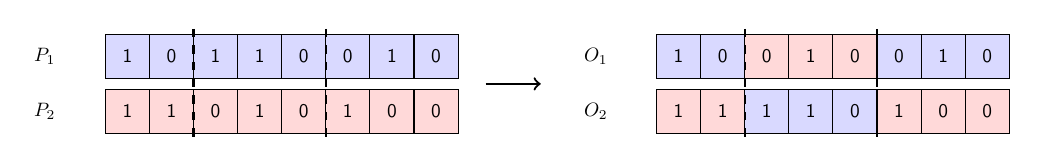
\begin{tikzpicture}[font=\sffamily, scale=0.7, transform shape]
\tikzstyle{bit}=[draw, minimum width=0.8cm, minimum height=0.8cm]
\tikzstyle{p1}=[bit, fill=blue!15]
\tikzstyle{p2}=[bit, fill=red!15]
\node at (-1.5, 1) {$P_1$};
\node[p1] at (0,1) {1}; \node[p1] at (0.8,1) {0}; \node[p1] at (1.6,1) {1}; \node[p1] at (2.4,1) {1}; \node[p1] at (3.2,1) {0}; \node[p1] at (4.0,1) {0}; \node[p1] at (4.8,1) {1}; \node[p1] at (5.6,1) {0};
\node at (-1.5, 0) {$P_2$};
\node[p2] at (0,0) {1}; \node[p2] at (0.8,0) {1}; \node[p2] at (1.6,0) {0}; \node[p2] at (2.4,0) {1}; \node[p2] at (3.2,0) {0}; \node[p2] at (4.0,0) {1}; \node[p2] at (4.8,0) {0}; \node[p2] at (5.6,0) {0};
\draw[->, thick] (6.5, 0.5) -- (7.5, 0.5);
\node at (8.5, 1) {$O_1$};
\node[p1] at (10,1) {1}; \node[p1] at (10.8,1) {0}; \node[p2] at (11.6,1) {0}; \node[p2] at (12.4,1) {1}; \node[p2] at (13.2,1) {0}; \node[p1] at (14.0,1) {0}; \node[p1] at (14.8,1) {1}; \node[p1] at (15.6,1) {0};
\node at (8.5, 0) {$O_2$};
\node[p2] at (10,0) {1}; \node[p2] at (10.8,0) {1}; \node[p1] at (11.6,0) {1}; \node[p1] at (12.4,0) {1}; \node[p1] at (13.2,0) {0}; \node[p2] at (14.0,0) {1}; \node[p2] at (14.8,0) {0}; \node[p2] at (15.6,0) {0};
\draw[dashed, thick] (1.2, 1.5) -- (1.2, -0.5);
\draw[dashed, thick] (3.6, 1.5) -- (3.6, -0.5);
\draw[dashed, thick] (11.2, 1.5) -- (11.2, -0.5);
\draw[dashed, thick] (13.6, 1.5) -- (13.6, -0.5);
\end{tikzpicture}
\caption{Ejemplo de funcionamiento del Cruce de dos puntos (2P).}
\label{fig:crossover_2p}
\end{figure}

    \item \textbf{Cruce Uniforme (\textit{Uniform Crossover} - UX):} A diferencia de los cruces por puntos de corte, el cruce uniforme \cite{syswerda1989uniform} trata cada gen de forma completamente independiente. Para cada posición, de forma aleatoria (con una probabilidad del $50\%$), se determina si los genes de los progenitores se intercambian o se mantienen, tal y como se esquematiza en la Figura \ref{fig:crossover_ux}. Este mecanismo elimina el sesgo posicional y maximiza la exploración individual, aunque presenta una mayor tendencia a romper secuencias de genes ya optimizadas.

\begin{figure}[H]
\centering
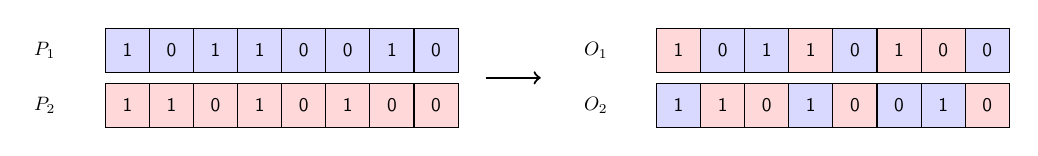
\begin{tikzpicture}[font=\sffamily, scale=0.7, transform shape]
\tikzstyle{bit}=[draw, minimum width=0.8cm, minimum height=0.8cm]
\tikzstyle{p1}=[bit, fill=blue!15]
\tikzstyle{p2}=[bit, fill=red!15]
\node at (-1.5, 1) {$P_1$};
\node[p1] at (0,1) {1}; \node[p1] at (0.8,1) {0}; \node[p1] at (1.6,1) {1}; \node[p1] at (2.4,1) {1}; \node[p1] at (3.2,1) {0}; \node[p1] at (4.0,1) {0}; \node[p1] at (4.8,1) {1}; \node[p1] at (5.6,1) {0};
\node at (-1.5, 0) {$P_2$};
\node[p2] at (0,0) {1}; \node[p2] at (0.8,0) {1}; \node[p2] at (1.6,0) {0}; \node[p2] at (2.4,0) {1}; \node[p2] at (3.2,0) {0}; \node[p2] at (4.0,0) {1}; \node[p2] at (4.8,0) {0}; \node[p2] at (5.6,0) {0};
\draw[->, thick] (6.5, 0.5) -- (7.5, 0.5);
\node at (8.5, 1) {$O_1$};
\node[p2] at (10,1) {1}; \node[p1] at (10.8,1) {0}; \node[p1] at (11.6,1) {1}; \node[p2] at (12.4,1) {1}; \node[p1] at (13.2,1) {0}; \node[p2] at (14.0,1) {1}; \node[p2] at (14.8,1) {0}; \node[p1] at (15.6,1) {0};
\node at (8.5, 0) {$O_2$};
\node[p1] at (10,0) {1}; \node[p2] at (10.8,0) {1}; \node[p2] at (11.6,0) {0}; \node[p1] at (12.4,0) {1}; \node[p2] at (13.2,0) {0}; \node[p1] at (14.0,0) {0}; \node[p1] at (14.8,0) {1}; \node[p2] at (15.6,0) {0};
\end{tikzpicture}
\caption{Ejemplo de funcionamiento del Cruce Uniforme (UX).}
\label{fig:crossover_ux}
\end{figure}

    \item \textbf{Cruce Medio Uniforme (\textit{Half Uniform Crossover} - HUX):} Variante especializada y altamente conservadora del cruce uniforme, propuesta por Eshelman \cite{eshelman1991chc}. Su funcionamiento se fundamenta en identificar primero y de forma exclusiva aquellos genes en los que ambos progenitores difieren. Durante la recombinación, se intercambia exactamente la mitad de estos genes distintos de manera aleatoria. Esta restricción garantiza que los descendientes hereden intacto todo el material genético en el que sus padres ya coincidían, y asegura que estos se sitúen geométricamente a la misma distancia de ambos progenitores. En la Figura \ref{fig:crossover_hux} se detalla este procedimiento, destacando la los genes que difieren en los progenitores.

\begin{figure}[H]
\centering
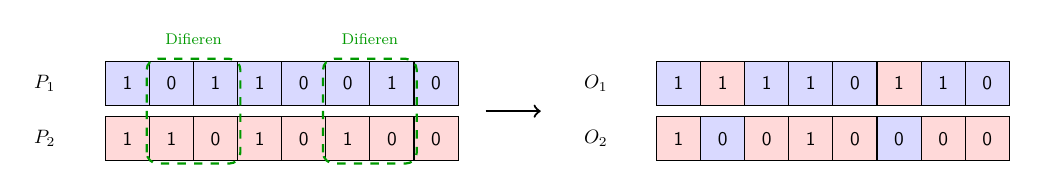
\begin{tikzpicture}[font=\sffamily, scale=0.7, transform shape]
\tikzstyle{bit}=[draw, minimum width=0.8cm, minimum height=0.8cm]
\tikzstyle{p1}=[bit, fill=blue!15]
\tikzstyle{p2}=[bit, fill=red!15]
\node at (-1.5, 1) {$P_1$};
\node[p1] at (0,1) {1}; \node[p1] at (0.8,1) {0}; \node[p1] at (1.6,1) {1}; \node[p1] at (2.4,1) {1}; \node[p1] at (3.2,1) {0}; \node[p1] at (4.0,1) {0}; \node[p1] at (4.8,1) {1}; \node[p1] at (5.6,1) {0};
\node at (-1.5, 0) {$P_2$};
\node[p2] at (0,0) {1}; \node[p2] at (0.8,0) {1}; \node[p2] at (1.6,0) {0}; \node[p2] at (2.4,0) {1}; \node[p2] at (3.2,0) {0}; \node[p2] at (4.0,0) {1}; \node[p2] at (4.8,0) {0}; \node[p2] at (5.6,0) {0};

% Marcar genes que difieren
\draw[green!60!black, thick, dashed, rounded corners] (0.35, -0.45) rectangle (2.05, 1.45);
\node[green!60!black, font=\footnotesize] at (1.2, 1.8) {Difieren};
\draw[green!60!black, thick, dashed, rounded corners] (3.55, -0.45) rectangle (5.25, 1.45);
\node[green!60!black, font=\footnotesize] at (4.4, 1.8) {Difieren};

\draw[->, thick] (6.5, 0.5) -- (7.5, 0.5);
\node at (8.5, 1) {$O_1$};
\node[p1] at (10,1) {1}; \node[p2] at (10.8,1) {1}; \node[p1] at (11.6,1) {1}; \node[p1] at (12.4,1) {1}; \node[p1] at (13.2,1) {0}; \node[p2] at (14.0,1) {1}; \node[p1] at (14.8,1) {1}; \node[p1] at (15.6,1) {0};
\node at (8.5, 0) {$O_2$};
\node[p2] at (10,0) {1}; \node[p1] at (10.8,0) {0}; \node[p2] at (11.6,0) {0}; \node[p2] at (12.4,0) {1}; \node[p2] at (13.2,0) {0}; \node[p1] at (14.0,0) {0}; \node[p2] at (14.8,0) {0}; \node[p2] at (15.6,0) {0};
\end{tikzpicture}
\caption{Ejemplo de funcionamiento del Cruce Medio Uniforme (HUX).}
\label{fig:crossover_hux}
\end{figure}
\end{itemize}

\section{Diseño experimental}

Para evaluar el rendimiento de los algoritmos seleccionados sobre el problema de la selección de etiquetas SNP, se propone un diseño experimental en el que se combinan de forma cruzada todos los algoritmos, estrategias de inicialización y operadores de cruce. Cada configuración única (algoritmo $\times$ inicialización $\times$ cruce) se replica múltiples veces para garantizar la robustez estadística de los resultados.

\subsection{Configuración de hiperparámetros comunes}

Los hiperparámetros globales compartidos por todos los algoritmos se han fijado de acuerdo con los valores empíricos habitualmente empleados en la literatura de MOEAs y de MaOEAs, y se detallan a continuación:

\begin{itemize}
    \item \textbf{Tamaño de población ($N_{pop}$):} 220 individuos.
    \item \textbf{Tamaño de la descendencia ($N_{desc}$):} 220 descendientes por generación.
    \item \textbf{Probabilidad de cruce ($p_c$):} 0,7.
    \item \textbf{Probabilidad de mutación ($p_m$):} $1/n$, donde $n = 772$ es el número de SNPs polimórficos efectivos del \textit{dataset}; de este modo se espera que se produzca, de media, exactamente una mutación por cromosoma.
    \item \textbf{Número de generaciones:} 500 generaciones por ejecución.
    \item \textbf{Modo de semillas:} Determinista, derivadas secuencialmente de una semilla maestra fija (42) para asegurar la reproducibilidad global de los experimentos.
    \item \textbf{Formulación de objetivos y normalización:} El diseño experimental contempla dos fases independientes para evaluar el impacto de la escala geométrica:
    \begin{enumerate}
        \item \textbf{Absoluta:} Objetivos evaluados en su escala natural, empleando límites fijos y estáticos derivados empíricamente del conjunto de datos para la normalización.
        \item \textbf{Proporcional:} Objetivos $f_3$ y $f_4$ divididos por $k$ y $k^2$ respectivamente, empleando límites estáticos proporcionales \cite{ting2010multi}.
    \end{enumerate}
    \item \textbf{Transformación geométrica:} Inversión de maximización a minimización mediante negación matemática ($f' = -f$).
    \item \textbf{Número de réplicas por configuración:} 31 ejecuciones independientes \cite{granado2020multiobjective}.
\end{itemize}

Además, se han definido los siguientes parámetros específicos para ciertos componentes del experimento:
\begin{itemize}
    \item Para la inicialización \textit{greedy\_multi}, se ha establecido un parámetro de \textit{tolerancia máxima objetivo} de 5, forzando de manera heurística la construcción de soluciones iniciales que distinguen cada par de haplotipos desde 1 hasta 5 veces.
    \item Para el algoritmo MOEA/D \cite{zhang2007moea}, los parámetros de vecindario son: número de vecinos $T = 15$ y probabilidad de cruce intra-vecindario $\delta = 0{,}9$.
\end{itemize}

El tamaño de población de 220 individuos se ha establecido con el objetivo de replicar de la forma más fiel posible las condiciones experimentales de Moqa \textit{et al.} \cite{moqa2022assessing}, quienes emplearon 200 individuos. Sin embargo, en algoritmos basados en descomposición, como NSGA-III \cite{deb2013evolutionary} y MOEA/D, la población debe coincidir con el número de vectores de referencia para garantizar un muestreo espacial uniforme. Dado que el método de Das y Dennis \cite{das1998normal} no puede generar exactamente 200 vectores simétricos para un problema de 4 objetivos ($M=4$), se seleccionó el resultado más aproximado. Utilizando $p=9$ particiones por eje, se generan exactamente $\binom{4+9-1}{9} = 220$ vectores de referencia, lo que fija, por consiguiente, el tamaño de la población.

\subsection{Factores de variación}

El estudio compara todas las combinaciones de los siguientes factores:

\begin{itemize}
    \item \textbf{Algoritmos:} SPEA2 \cite{zitzler2001spea2}, NSGA-II \cite{deb2002fast}, NSGA-III \cite{deb2013evolutionary}, U-NSGA-III \cite{seada2015unified}, MOEA/D \cite{zhang2007moea}, AGE-MOEA-II \cite{panichella2022adaptive}, SMS-EMOA \cite{beume2007sms} y RVEA \cite{cheng2016reference}.
    \item \textbf{Estrategias de inicialización:} \textit{random\_dense} \cite{ting2010multi}, \textit{greedy\_ting} \cite{ting2010multi} y \textit{greedy\_multi}.
    \item \textbf{Operadores de cruce:} UX \cite{syswerda1989uniform}, HUX \cite{eshelman1991chc}, 1P y 2P \cite{holland1975adaptation}.
\end{itemize}

Esto da lugar a un total de $8 \times 3 \times 4 = 96$ configuraciones distintas. Dado que se realizan 31 réplicas independientes \cite{granado2020multiobjective} por cada configuración y se llevan a cabo dos experimentos (absoluto y proporcional), el estudio abarca un total de 5952 ejecuciones independientes.

\subsection{Normalización}

La optimización de la selección de etiquetas SNP presenta un problema de escala, ya que los diferentes objetivos operan en rangos numéricos distintos. En el experimento de objetivos proporcionales, mientras que la \textit{Compacidad} ($f_1$) varía en un rango teórico de $[1, 772]$, otros objetivos operan en órdenes de magnitud fraccionales, como el \textit{Balance} ($f_4$), cuyo rango queda acotado al intervalo $[0, 0.25]$. Esta divergencia teórica, donde el límite máximo de un objetivo supera por un factor de $3 \times 10^3$ a la dimensión de otro, provoca que normalizar el espacio de búsqueda sea un requisito metodológico obligatorio para poder estandarizar la evaluación estadística posterior.

El cálculo equitativo de las métricas de rendimiento de los algoritmos, como el hipervolumen \cite{zitzler1999multiobjective}, exige un espacio matemático uniforme y acotado. Si los objetivos se evalúan en su escala natural, el cálculo del área geométrica cubierta sesgaría inevitablemente los resultados de las métricas, favoreciendo de forma artificial a aquellas soluciones que despuntan en la dimensión de mayor escala, lo cual invalidaría cualquier comparativa empírica.

Para abordar este problema, los frentes se escalan al espacio unitario cerrado $[0, 1]$ utilizando límites fijos precalculados a partir del conjunto de datos. Para cada uno de los experimentos se aplicó una normalización diferente, estructurada de la siguiente forma:

\begin{enumerate}
    \item \textbf{Normalización absoluta (\texttt{static\_dataset\_limits}):} Bajo este esquema, utilizado en el experimento de objetivos absolutos, los objetivos se evalúan en su escala física natural original. La normalización se realiza calculando los puntos ideal ($Z^*$) y nadir ($Z^{nad}$) teóricos de forma estática a partir de las propiedades estructurales del \textit{dataset} completo, siendo $L$ el número total de SNPs polimórficos. De este modo, los vectores de referencia quedan definidos como:
    \begin{itemize}
        \item Punto Ideal ($Z^*$): $\left[1,\ -L,\ -\left(\frac{1}{|P|} \sum_{(h_i, h_j) \in P} d_H(h_i, h_j)\right),\ 0\right]$
        \item Punto Nadir ($Z^{nad}$): $\left[L,\ 0,\ 0,\ \frac{L^2}{4}\right]$
    \end{itemize}
    \textit{(Donde $P$ es el conjunto de todos los pares de haplotipos posibles y $d_H$ denota la distancia de Hamming).}

    \item \textbf{Normalización proporcional (\texttt{static\_proportional\_limits}):} En esta alternativa, empleada en el experimento de objetivos proporcionales, los objetivos $f_3$ y $f_4$ se transforman: la \textit{Disimilitud} ($f_3$) se divide por la \textit{Compacidad} ($f_1$), que representa el número de etiquetas SNP seleccionados; y el \textit{Balance} (varianza) se divide por el cuadrado de dicho objetivo ($f_1^2$). La tolerancia ($f_2$) se excluye de esta transformación y mantiene su límite absoluto. Debido a estas modificaciones, la normalización utiliza topes geométricos fraccionales, quedando los vectores de referencia definidos como:
    \begin{itemize}
        \item Punto Ideal ($Z^*$): $\left[1,\ -L,\ -1{,}0,\ 0\right]$
        \item Punto Nadir ($Z^{nad}$): $\left[L,\ 0,\ 0,\ 0{,}25\right]$
    \end{itemize}
\end{enumerate}



En resumen, el uso de estos límites estáticos extraídos del dataset es indispensable para evaluar rigurosamente el rendimiento mediante métricas estadísticas en un estudio que consta de 2 experimentos (uno mediante formulación de objetivos absoluta y otro proporcional). Si la normalización se realizase basándose en los resultados de cada experimento (extrayendo los valores máximos y mínimos descubiertos por toda la batería de algoritmos de un experimento), el tamaño del espacio matemático variaría en cada uno de ellos. Las fluctuaciones estocásticas en las soluciones encontradas desplazarían las fronteras geométricas, lo que invalidaría por completo la comparación de métricas (como el hipervolumen) entre ambos. Al definir vectores de referencia teóricos e inmutables, extraídos del dataset, se asegura que el espacio normalizado sea siempre idéntico, garantizando una comparativa analítica justa bajo las mismas condiciones espaciales.

\subsection{Métricas de evaluación}

Siguiendo y ampliando las métricas usadas por Ting \textit{et al.} \cite{ting2010multi} y por Moqa \textit{et al.} \cite{moqa2022assessing}, se emplean las siguientes que evalúan la calidad de los frentes de Pareto resultantes:

\subsubsection{Métricas de Rendimiento Integral}

Son aquellas que dictan el rendimiento global, evaluando convergencia y diversidad al mismo tiempo.

\begin{itemize}
    \item \textbf{Hipervolumen (HV) (a maximizar):} Mide el volumen del espacio objetivo dominado por el frente respecto al punto de referencia $[1{,}1; 1{,}1; 1{,}1; 1{,}1]$ en el espacio normalizado \cite{zitzler1999multiobjective}. Integra simultáneamente la convergencia y la diversidad de las soluciones obtenidas. En la Figura \ref{fig:metric_hypervolume}, se compara la cobertura geométrica de dos frentes bidimensionales. El Algoritmo A, al presentar soluciones extremas bien distribuidas (alcanzando los ejes en $0{,}0$ y $1{,}0$) y converger cerca del origen, logra maximizar el área dominada (sombreada). En contraste, el Algoritmo B genera soluciones concentradas y subóptimas, dejando vastas porciones del espacio objetivo sin cubrir, lo que resulta en un HV mermado.

\begin{figure}[H]
    \centering
    \includegraphics[width=1\textwidth]{../figuras_metricas/hypervolume_metric.pdf}
    \caption[Cálculo de la métrica de Hipervolumen]{Ejemplo analítico y visual del cálculo de la métrica de Hipervolumen. El panel izquierdo demuestra cómo una alta convergencia combinada con una distribución amplia (incluyendo extremos) logra maximizar el área sombreada respecto al punto de referencia ($1{,}1; 1{,}1$). El panel derecho revela el impacto negativo de obtener soluciones poco diversas y alejadas del óptimo.}
    \label{fig:metric_hypervolume}
\end{figure}

    \item \textbf{Inverted Generational Distance Plus (IGD+) (a minimizar):} Indicador de convergencia y diversidad relativa al frente de referencia empírico \cite{ishibuchi2015igd}, construido como la unión no dominada de todos los frentes finales del experimento. Para clarificar la distinción teórica de su cálculo geométrico respecto a GD+ (véase la Figura \ref{fig:metric_igd}), la métrica \textbf{IGD+} invierte la perspectiva y mide la distancia \textit{desde} cada punto del frente de referencia empírico \textit{hacia} la solución descubierta más cercana. Este enfoque evalúa de forma conjunta la convergencia y la diversidad: aunque las soluciones del algoritmo sean localmente precisas, si se omiten regiones enteras del espacio de búsqueda, los puntos óptimos inexplorados generarán vectores de distancia largos que empeorarán drásticamente el valor numérico final.

\begin{figure}[H]
    \centering
    \includegraphics[width=0.6\textwidth]{../figuras_metricas/igd_metric.pdf}
    \caption[Cálculo geométrico diferencial de IGD+]{Esquema diferencial del cálculo geométrico de IGD+. Demuestra la medición inversa desde el frente empírico de referencia hacia las soluciones descubiertas, penalizando estructuralmente la falta de convergencia y también la diversidad del algoritmo.}
    \label{fig:metric_igd}
\end{figure}
\end{itemize}

\subsubsection{Métricas Geométricas Puras}

Evalúan de forma aislada la convergencia o la diversidad.

\begin{itemize}
    \item \textbf{Generational Distance Plus (GD+) (a minimizar):} Como complemento al indicador anterior, la métrica \textbf{GD+} mide la distancia analítica \textit{desde} las soluciones descubiertas por el algoritmo \textit{hacia} el frente de referencia empírico. Actúa como un indicador de convergencia estricta: penaliza severamente si alguna solución descubierta es de mala calidad y se ubica lejos del frente de referencia empírico, sin tener en cuenta la dispersión de las mismas.

\begin{figure}[H]
    \centering
    \includegraphics[width=0.6\textwidth]{../figuras_metricas/gd_metric.pdf}
    \caption[Cálculo geométrico diferencial de GD+]{Esquema diferencial del cálculo geométrico de GD+. Ilustra la medición desde las soluciones descubiertas hacia la referencia, evaluando únicamente la convergencia.}
    \label{fig:metric_gd}
\end{figure}
    
    \item \textbf{Rango (a maximizar):} Suma de los rangos por objetivo del frente normalizado; valora la diversidad geométrica global y puramente la expansión del frente de Pareto en los ejes extremos. Para ilustrar este concepto analítica y visualmente (véase la Figura \ref{fig:metric_range}), se representa un escenario bidimensional. El frente de alta diversidad (círculos azules) distribuye sus soluciones abarcando desde la coordenada $1{,}0$ hasta la $6{,}0$ en ambos ejes. Esto resulta en una amplitud de $5{,}0$ unidades por objetivo, sumando un \textit{Range} global de $10{,}0$. En contraposición, el frente de baja diversidad (cuadrados rojos) presenta soluciones atrapadas en una región estrecha, abarcando únicamente desde $3{,}5$ hasta $4{,}2$ en el eje $f_1$, y desde $3{,}8$ hasta $4{,}5$ en el eje $f_2$. Al colapsar sus proyecciones hacia rangos de tan solo $0{,}7$ unidades por objetivo, su métrica final se desploma a un valor escalar de $1{,}4$, evidenciando matemáticamente la escasez de variedad en las opciones descubiertas.

\begin{figure}[H]
    \centering
    \includegraphics[width=0.75\textwidth]{../figuras_metricas/range_metric.pdf}
    \caption[Representación geométrica de la métrica Range]{Representación geométrica bidimensional de la métrica Range. Se contrasta analíticamente la proyección espacial de un frente con alta amplitud (círculos azules) frente a una agrupación de soluciones con baja dispersión (cuadrados rojos).}
    \label{fig:metric_range}
\end{figure}
\end{itemize}

\subsubsection{Métricas de Topología Local}

Evalúan la calidad de las soluciones individuales clave, independientemente del volumen del conjunto.

\begin{itemize}
    \item \textbf{Convergencia Marginal (SumMin) (a minimizar):} Suma de los mejores valores alcanzados en cada objetivo; evalúa qué configuración ha encontrado las soluciones más extremas en cada eje de manera marginal.
    
    \item \textbf{Balance Central (MinSum) (a minimizar):} Valor mínimo de la suma de objetivos del frente; evalúa qué configuración es capaz de encontrar la solución más equilibrada que contenta a todos los objetivos al mismo tiempo.

    Para ilustrar analíticamente la diferencia teórica entre ambas métricas de topología (véase la Tabla \ref{tab:metric_sum}), se expone un frente normalizado hipotético compuesto por tres soluciones evaluadas en cuatro objetivos a minimizar.

\begin{table}[H]
    \centering
    \begin{tabular}{lcccc|c}
        \hline
        \textbf{Solución} & \textbf{$f_1$} & \textbf{$f_2$} & \textbf{$f_3$} & \textbf{$f_4$} & \textbf{Suma Total ($\sum f_i$)} \\
        \hline
        $S_1$ & $\mathbf{0{,}1}$ & $0{,}8$ & $0{,}6$ & $0{,}5$ & $2{,}0$ \\
        $S_2$ & $0{,}4$ & $\mathbf{0{,}2}$ & $0{,}7$ & $\mathbf{0{,}3}$ & $\mathbf{1{,}6}$ \\
        $S_3$ & $0{,}9$ & $0{,}5$ & $\mathbf{0{,}1}$ & $0{,}6$ & $2{,}1$ \\
        \hline
    \end{tabular}
    \caption[Evaluación analítica de SumMin y MinSum]{Ejemplo analítico para la evaluación de SumMin y MinSum. El cálculo de SumMin requiere la extracción de los mínimos marginales (resaltados en negrita en cada columna de los objetivos), resultando en la suma $0{,}1 + 0{,}2 + 0{,}1 + 0{,}3 = 0{,}7$. En contraposición, el cálculo de MinSum requiere identificar la única solución con mejor balance general, lo que equivale a seleccionar el valor mínimo de la última columna ($1{,}6$, correspondiente a $S_2$).}
    \label{tab:metric_sum}
\end{table}
\end{itemize}

\subsubsection{Métricas de Dominio Biológico}

Métricas específicas del problema que demuestran la utilidad real de las soluciones encontradas.

\begin{itemize}
    \item \textbf{Tasas de Eficiencia de Tolerancia (\textit{MaxToleranceRate}, \textit{AvgToleranceRate}) (a maximizar):} Métricas de dominio específico que cuantifican la tolerancia ($f_2$) en proporción a la compacidad ($f_1$). Como se ilustra analíticamente (véase la Figura \ref{fig:metric_tolerance}), estas métricas dividen la tolerancia neta ($f_2$) entre la compacidad ($f_1$) para obtener la eficiencia de la tolerancia. \textit{MaxToleranceRate} captura el pico máximo de eficiencia a lo largo del frente, revelando la configuración algorítmica con mejor rentabilidad coste-seguridad. Por su parte, \textit{AvgToleranceRate} promedia todas las tasas obtenidas, proporcionando una evaluación global sobre la capacidad del algoritmo para mantener soluciones altamente eficientes.

\begin{figure}[H]
    \centering
    \includegraphics[width=1\textwidth]{../figuras_metricas/tolerance_rate_metric.pdf}
    \caption[Cálculo de métricas de eficiencia de tolerancia]{Ejemplo visual y analítico del cálculo de las métricas de eficiencia de la tolerancia. El panel izquierdo ilustra un frente de Pareto evaluando Compacidad ($f_1$) frente a Tolerancia ($f_2$), indicando la Tasa de Tolerancia ($TR$) en cada nodo. El panel derecho muestra la distribución de estas tasas, identificando gráficamente el valor pico (\textit{MaxToleranceRate}) y la media aritmética (\textit{AvgToleranceRate}).}
    \label{fig:metric_tolerance}
\end{figure}

    \item \textbf{Distancia de Hamming Promedio (\textit{AvgHammingDistance}) (a maximizar):} Indicador del rendimiento global del frente de Pareto respecto al tercer objetivo del problema ($f_3$). Sirve para comprobar cómo se comporta la población algorítmica manteniendo la diversidad genotípica promedio de la muestra. Se calcula como la media aritmética del valor del objetivo de disimilitud a través de todas las soluciones que componen el frente.
    \begin{equation}
        AvgHammingDistance = \frac{1}{|P|} \sum_{s \in P} f_3(s)
    \end{equation}
    donde $|P|$ representa la cardinalidad del frente de Pareto y $f_3(s)$ es el valor de la distancia media de Hamming evaluada para la solución $s$.
\end{itemize}

\subsection{Análisis estadístico}

Dado el carácter estocástico de los algoritmos evolutivos, los resultados de las 31 réplicas independientes \cite{granado2020multiobjective} de cada configuración se someten a un análisis estadístico inferencial no paramétrico para validar empíricamente las diferencias de rendimiento. Para evaluar el desempeño en cada uno de los indicadores aislados, se aplica la prueba ómnibus de Kruskal-Wallis \cite{kruskal1952use}. En caso de detectarse diferencias significativas globales, se emplea el test \textit{post-hoc} de Dunn \cite{dunn1964multiple} para identificar la significancia estadística entre pares específicos de configuraciones.

En todas las pruebas inferenciales de este estudio se establece un nivel de significancia estricto de $\alpha = 0{,}05$.

\subsection{Representación de frentes de Pareto}

Para el análisis visual de los frentes de Pareto obtenidos por cada algoritmo evolutivo, se emplea un proceso de agregación de resultados. Debido al carácter estocástico de estas técnicas, la representación gráfica se construye uniendo la réplica con el valor mediano en la métrica de hipervolumen \cite{knowles2006tutorial} de todas las configuraciones evaluadas para un mismo algoritmo (tres estrategias de inicialización poblacional y cuatro operadores de cruce), resultando de este modo en un total de 8 gráficas.

Dado que el problema de selección de etiquetas SNP consta de cuatro objetivos, su representación directa resulta inviable. Por consiguiente, se utilizan proyecciones bidimensionales cruzadas para facilitar la interpretación geométrica del espacio de soluciones. Concretamente, la figura asociada a cada algoritmo se desglosa en seis gráficas bidimensionales (como se ilustra de manera ejemplificada en la Figura \ref{fig:pareto_front_example}), correspondientes a todas las combinaciones pareadas posibles de los objetivos. Adicionalmente, se superponen curvas de regresión local \textit{LOWESS} (\textit{Locally Weighted Scatterplot Smoothing}) \cite{cleveland1979robust} sobre los datos proyectados. Estas curvas abstraen la tendencia del comportamiento del algoritmo, mitigando el impacto visual de la dispersión de las soluciones.

\begin{figure}[H]
    \centering
    \includegraphics[width=\textwidth]{"../../exp/full_31/ABS 20260625T071958/2_comparativa/1_frentes/frentes_pareto/frentes_pareto_agregados_nsga2_full_31.png"}
    \caption[Disposición gráfica de los frentes de Pareto]{Ejemplo ilustrativo de la disposición geométrica para el análisis de resultados. Se muestra una matriz de seis proyecciones bidimensionales correspondientes a todas las combinaciones pareadas de los cuatro objetivos, acompañadas por sus respectivas curvas de tendencia LOWESS. Los datos numéricos y algorítmicos concretos de este ejemplo no son objeto de análisis en esta sección metodológica.}
    \label{fig:pareto_front_example}
\end{figure}
